%% 
%% Copyright 2007-2025 Elsevier Ltd
%% 
%% This file is part of the 'Elsarticle Bundle'.
%% ---------------------------------------------
%% 
%% Template article for Elsevier's document class `elsarticle'
%% with harvard style bibliographic references

\documentclass[preprint,12pt]{elsarticle}

%% The amssymb package provides various useful mathematical symbols
\usepackage{amssymb}
\usepackage{float}

%% The amsmath package provides various useful equation environments.
\usepackage{amsmath}
\usepackage{graphicx}
\usepackage{hyperref}

\begin{document}

\begin{frontmatter}
%% Title
\title{PythonSLM: A Specialized Small Language Model for Python Code Generation}

%% Authors
\author{Satyam Kumar Chauhan (123108031)}
\author{Venkatesh Shukla (123108030)}
\author{Jayant Gautam (123108039)}
\author{Aditya Rai (123108034)}

\end{frontmatter}

%% main text
\section{Background}

Recent advances in large language models have revolutionized code generation and programming assistance. Models like GPT-4, CodeLlama, and StarCoder demonstrate impressive capabilities across various programming tasks. However, these models typically contain billions of parameters, requiring expensive cloud infrastructure and making them impractical for local deployment on consumer hardware.

Despite their effectiveness, general-purpose code models are trained across multiple programming languages, which can dilute their performance on language-specific patterns and idioms. For Python specifically, this means missing out on Pythonic conventions and best practices that are crucial for generating high-quality code.

Recent research has shown that smaller, specialized models can achieve competitive performance when trained with focused datasets and careful optimization. Work on models like Phi-1 and Phi-2 \citep{gunasekar2023phi} demonstrates that models with around 1.3B parameters trained on high-quality, curated data can match larger models on reasoning tasks. Similarly, DistilBERT \citep{sanh2019distilbert} shows that compact models can retain significant performance through knowledge distillation. Models with 300-500 million parameters can be both powerful and practical for local deployment, offering an opportunity to develop lightweight code assistants that excel in specific programming languages while remaining accessible.

\section{Objective}

The objective of this project is to develop a specialized Small Language Model (SLM) optimized for Python code generation and understanding. We aim to demonstrate that a compact model with 300-500 million parameters can achieve strong performance on Python-specific tasks while being efficient enough for local deployment.

Specifically, this work focuses on:
\begin{itemize}
\item Building or adapting a lightweight transformer-based architecture
\item Training on curated, high-quality Python code datasets
\item Optimizing for Python-specific syntax and idiomatic patterns
\item Evaluating performance on standard benchmarks like HumanEval
\item Ensuring local execution on consumer hardware without cloud dependency
\end{itemize}

\section{Problem Statement}

Current state-of-the-art code models are multi-billion parameter systems requiring expensive infrastructure, making them inaccessible for local use and raising privacy concerns for developers working with proprietary code. General-purpose models trained across numerous languages often lack deep specialization in Python-specific patterns.

The computational demands of large models create barriers for students, researchers, and developers in resource-constrained environments. There's a clear need for lightweight, specialized alternatives that democratize access to AI-powered programming assistance.

Therefore, the core research question is:

\textit{Can a specialized Small Language Model with 300-500 million parameters, trained exclusively on Python code, achieve competitive performance while remaining efficient enough for local deployment on consumer hardware?}

\section{Research Gap and Novelty}

Existing research has primarily focused on scaling up model size or training large general-purpose models. Limited work explores building specialized small models from scratch for a single programming language.

This project's novelty lies in:
\begin{itemize}
\item \textbf{Language Specialization:} Exclusive focus on Python enables deeper learning of language-specific patterns without multi-language training dilution
\item \textbf{Local Deployment:} Prioritizing inference efficiency for consumer hardware
\item \textbf{Curated Training:} Combining multiple high-quality Python datasets covering diverse scenarios
\end{itemize}

\section{Social Impact and Real-World Relevance}

A lightweight, locally-deployable Python model democratizes access to AI programming assistance. For students and learners, it enables coding education without expensive cloud services, particularly valuable in regions with limited resources. For professional developers, local deployment offers privacy-preserving code assistance for proprietary codebases.

This project also contributes to sustainable AI practices by demonstrating that smaller models can achieve strong performance, reducing the carbon footprint of both training and inference. An open approach fosters a diverse ecosystem of specialized tools, reducing dependence on large closed-source models.

\section{Dataset Description}

\subsection{Core Training Datasets}

\subsubsection{CodeSearchNet (Python Subset)}
A large-scale dataset with Python functions from GitHub repositories paired with documentation, providing real-world code examples.
\begin{itemize}
\item \textbf{Task:} Code-documentation alignment, function generation
\item \textbf{Scale:} ~1.3 million Python functions
\end{itemize}

\subsubsection{APPS Dataset}
Coding problems spanning introductory to competitive programming levels with test cases.
\begin{itemize}
\item \textbf{Task:} Algorithmic problem solving
\item \textbf{Scale:} 10,000 problems with difficulty ratings
\end{itemize}

\subsubsection{MBPP Dataset}
Entry-level programming problems testing basic Python skills.
\begin{itemize}
\item \textbf{Task:} Basic programming and function implementation
\item \textbf{Scale:} 974 programming problems
\end{itemize}

\subsubsection{CodeContests Dataset}
Competitive programming problems from platforms like Codeforces.
\begin{itemize}
\item \textbf{Task:} Advanced algorithmic programming
\item \textbf{Scale:} Thousands of contest problems
\end{itemize}

\subsubsection{The Stack (Python-Filtered)}
Large-scale, clean Python code from open-source repositories.
\begin{itemize}
\item \textbf{Task:} General Python code understanding
\item \textbf{Scale:} Multiple gigabytes of filtered code
\end{itemize}

\subsection{Evaluation Dataset}

\subsubsection{HumanEval}
A benchmark with 164 hand-written programming problems for evaluating code generation.

\section{Related Work}

\subsection{Large Language Models for Code}
Models like Codex \citep{chen2021codex}, CodeLlama \citep{roziere2023codellama}, and StarCoder \citep{li2023starcoder} achieve state-of-the-art performance through scale. However, with 7B+ parameters, they're computationally expensive and impractical for local use.

\subsection{Multimodal and Reasoning-Focused LLMs}
Recent work has also explored improving reasoning and multistep problem solving in multimodal language models. Anand et al. \citep{anand2024geometry} introduce a geometry-focused multimodal benchmark and evaluation framework designed to test structured reasoning, multistep scoring, and visual-textual understanding. Their work highlights that domain-focused datasets and targeted evaluation pipelines can significantly improve reasoning performance in specialized settings.

\subsection{Small and Efficient Models}
Work on DistilBERT \citep{sanh2019distilbert} and TinyBERT \citep{jiao2020tinybert} shows that knowledge distillation creates compact models retaining performance. Phi-1 and Phi-2 \citep{gunasekar2023phi} demonstrate that small models trained on high-quality data can achieve impressive results, suggesting careful curation matters more than pure scale.

\section{Data Cleaning}

Preprocessing steps applied uniformly across datasets:
\begin{itemize}
\item Syntax validation
\item Length filtering to maintain reasonable token distributions
\item License filtering for permissive open-source content
\item Consistent formatting while preserving meaningful whitespace
\end{itemize}

% EDA
\section{Exploratory Data Analysis}

Exploratory Data Analysis (EDA) is performed to understand dataset characteristics and potential challenges prior to model training.

\subsection{Statistical Analysis}

\begin{itemize}
    \item Distribution of code lengths across datasets (mean, median, maximum)
    \item Token count estimation
    \item Problem difficulty distribution in APPS dataset
    \item Dataset composition and sample counts
\end{itemize}

\subsection{Key Findings}

Code length analysis reveals distinct patterns across datasets:
\begin{itemize}
\item MBPP: median 10 lines (entry-level problems)
\item CodeSearchNet: median 24 lines (typical functions)
\item The Stack: median 32 lines (diverse structures)
\item APPS: median 45 lines (algorithmic solutions)
\item CodeContests: median 68 lines (complex competitions)
\end{itemize}

The training corpus comprises 1.8 million Python samples. CodeSearchNet (71.5\%, 1.3M) and The Stack (27.5\%, 500K) provide large-scale real-world code, while APPS (10K), CodeContests (13K), and MBPP (974) contribute specialized algorithmic examples.

APPS dataset shows balanced difficulty: Introductory (40\%), Interview (35\%), Competition (25\%), ensuring exposure across complexity levels.

\subsection{Statistical Summary}

\begin{table}[h]
\centering
\caption{Code Length Statistics (Lines of Code)}
\label{tab:stats_summary}
\small
\begin{tabular}{lcccccc}
\hline
\textbf{Dataset} & \textbf{Mean} & \textbf{Median} & \textbf{Std Dev} & \textbf{Min} & \textbf{Max} & \textbf{75th Percentile} \\
\hline
MBPP & 12.3 & 10.0 & 8.2 & 3 & 45 & 16 \\
CodeSearchNet & 28.7 & 24.0 & 18.5 & 5 & 120 & 38 \\
The Stack & 38.2 & 32.0 & 24.1 & 8 & 180 & 52 \\
APPS & 58.4 & 45.0 & 35.7 & 12 & 250 & 75 \\
CodeContests & 84.6 & 68.0 & 52.3 & 20 & 350 & 110 \\
\hline
\end{tabular}
\end{table}

\subsection{Visualizations}

The following visualizations are generated as part of EDA:
\begin{itemize}
    \item Histogram of code length distributions across all datasets
    \item Bar chart showing dataset sizes
    \item Distribution of problem difficulties in APPS dataset
\end{itemize}

\subsection{EDA Figures}

Figures obtained from EDA are shown below.

\subsubsection{Dataset Sizes}
Analysis of dataset composition shows CodeSearchNet and The Stack dominate the training corpus with 1.3M and 500K samples respectively. The remaining datasets (APPS, CodeContests, MBPP) contribute specialized algorithmic examples totaling approximately 24K samples.

\begin{figure}[H]
    \centering
    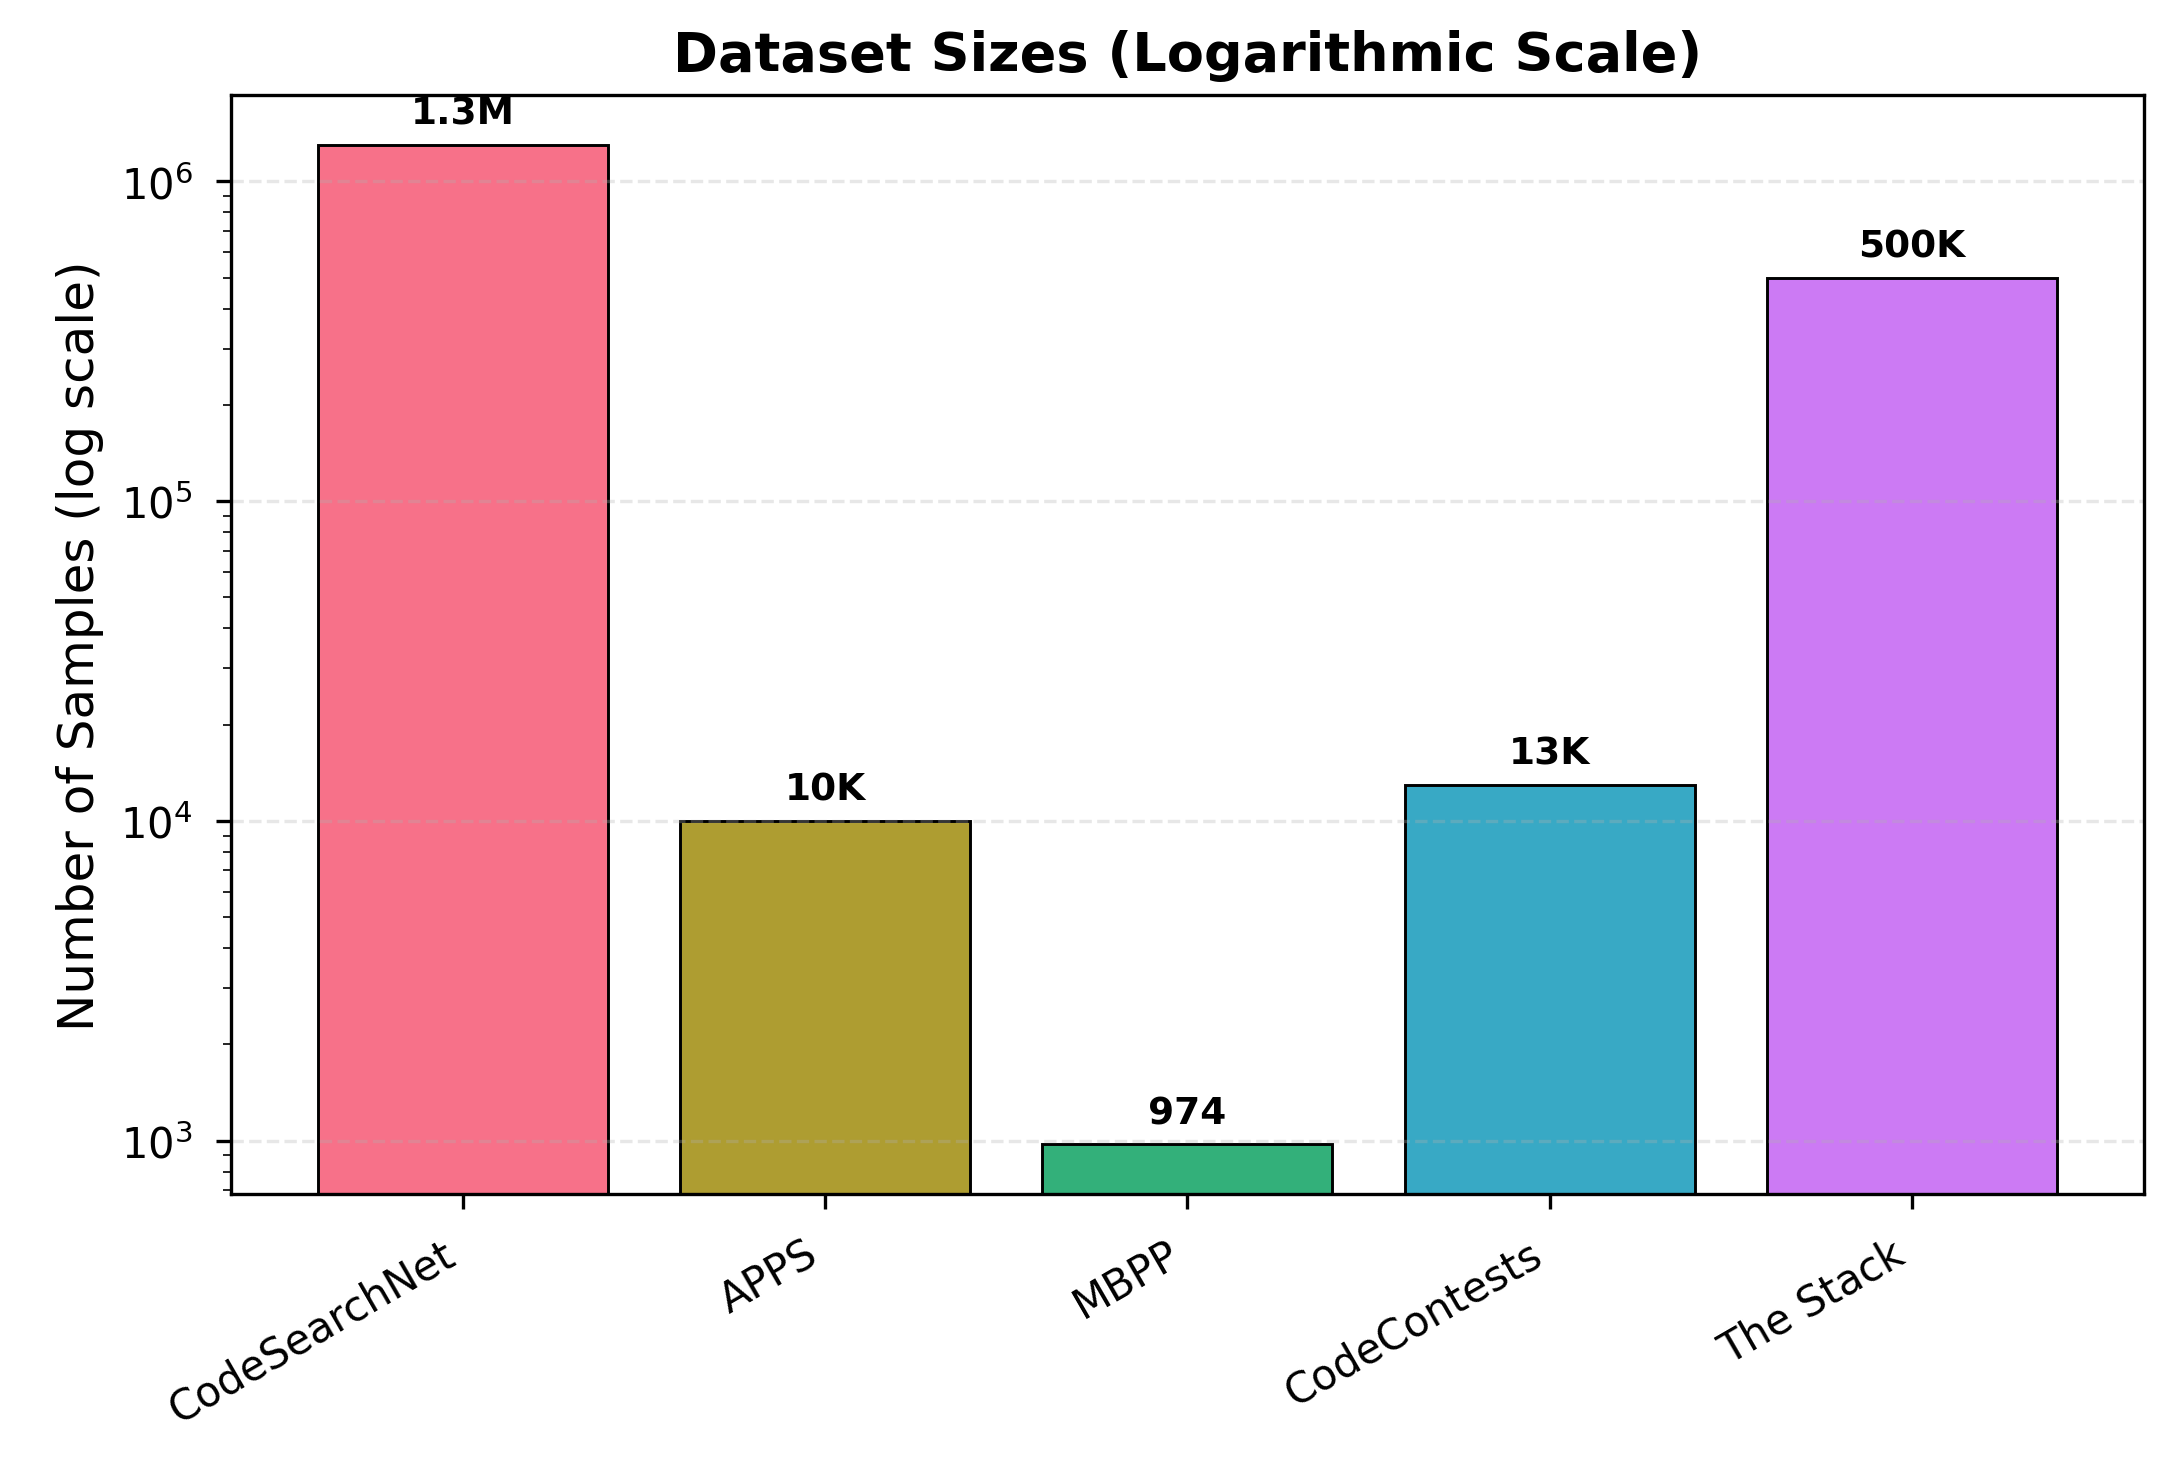
\includegraphics[width=0.8\textwidth]{dataset_composition.png}
    \caption{Dataset Sizes Across Training Corpus}
\end{figure}

\subsubsection{Code Length Distribution}
The distribution reveals varying complexity levels across datasets. MBPP exhibits the shortest code samples suitable for basic programming tasks, while CodeContests shows the longest implementations reflecting competitive programming complexity.

\begin{figure}[H]
    \centering
    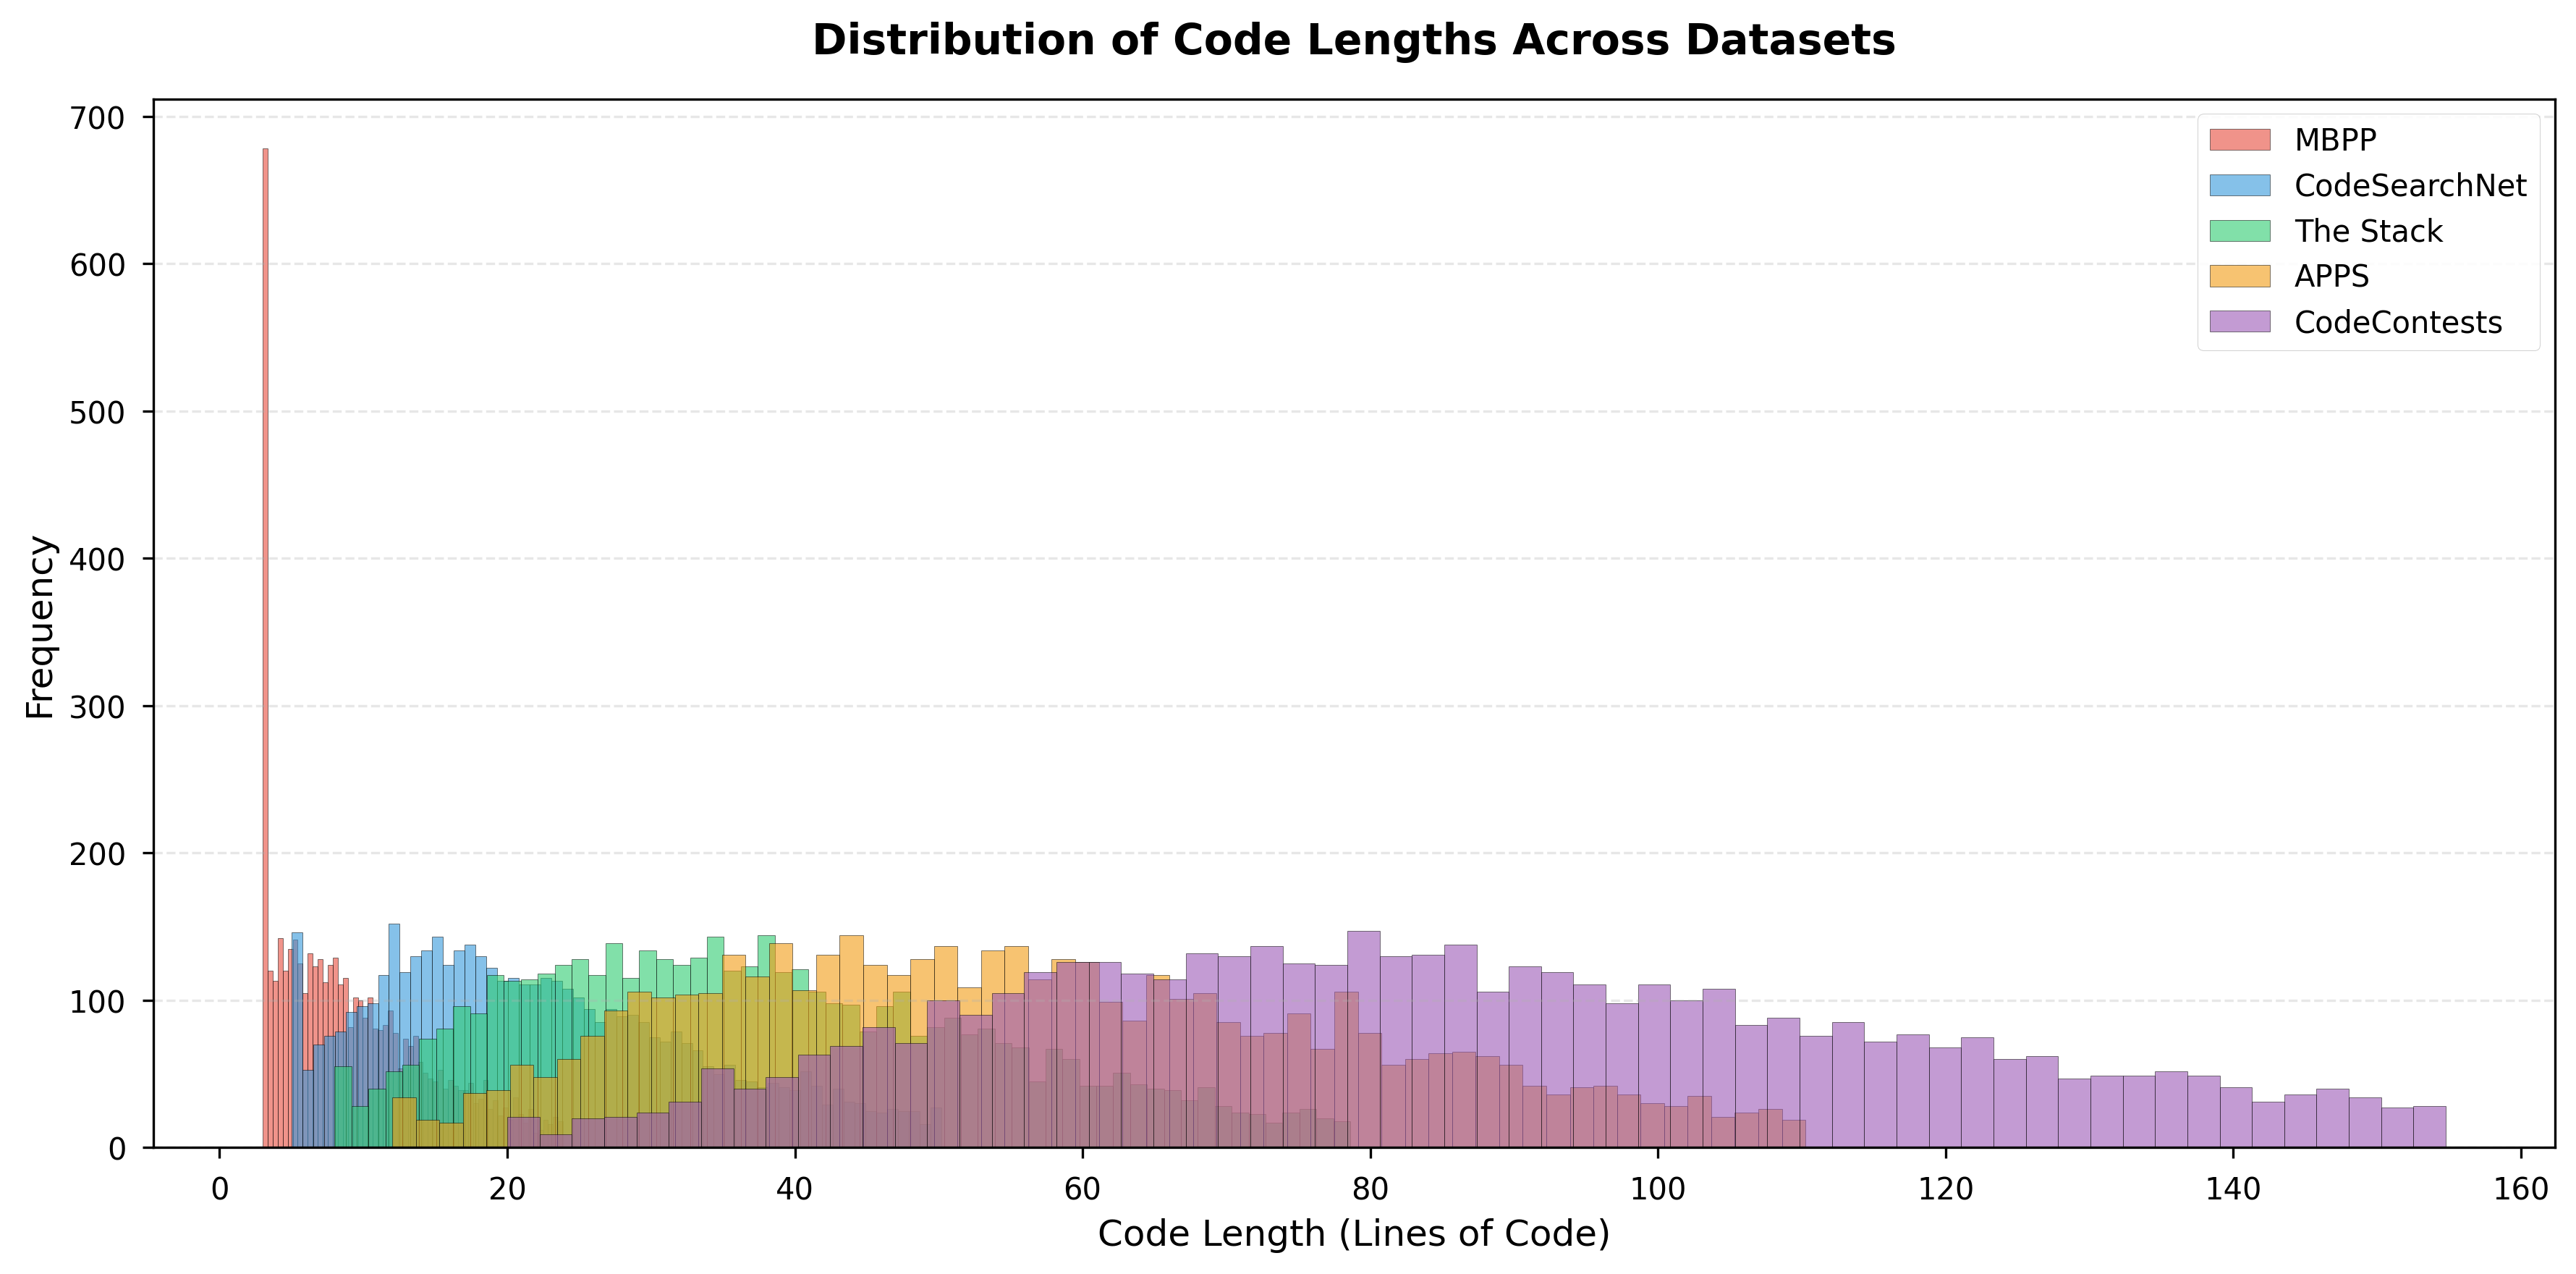
\includegraphics[width=0.8\textwidth]{code_length_distribution.png}
    \caption{Distribution of Code Lengths Across Datasets}
\end{figure}

\subsubsection{Problem Difficulty Analysis}
The APPS dataset maintains a balanced distribution across difficulty levels, with introductory problems comprising the largest portion (40\%), followed by interview-level (35\%) and competition-level problems (25\%).

\begin{figure}[H]
    \centering
    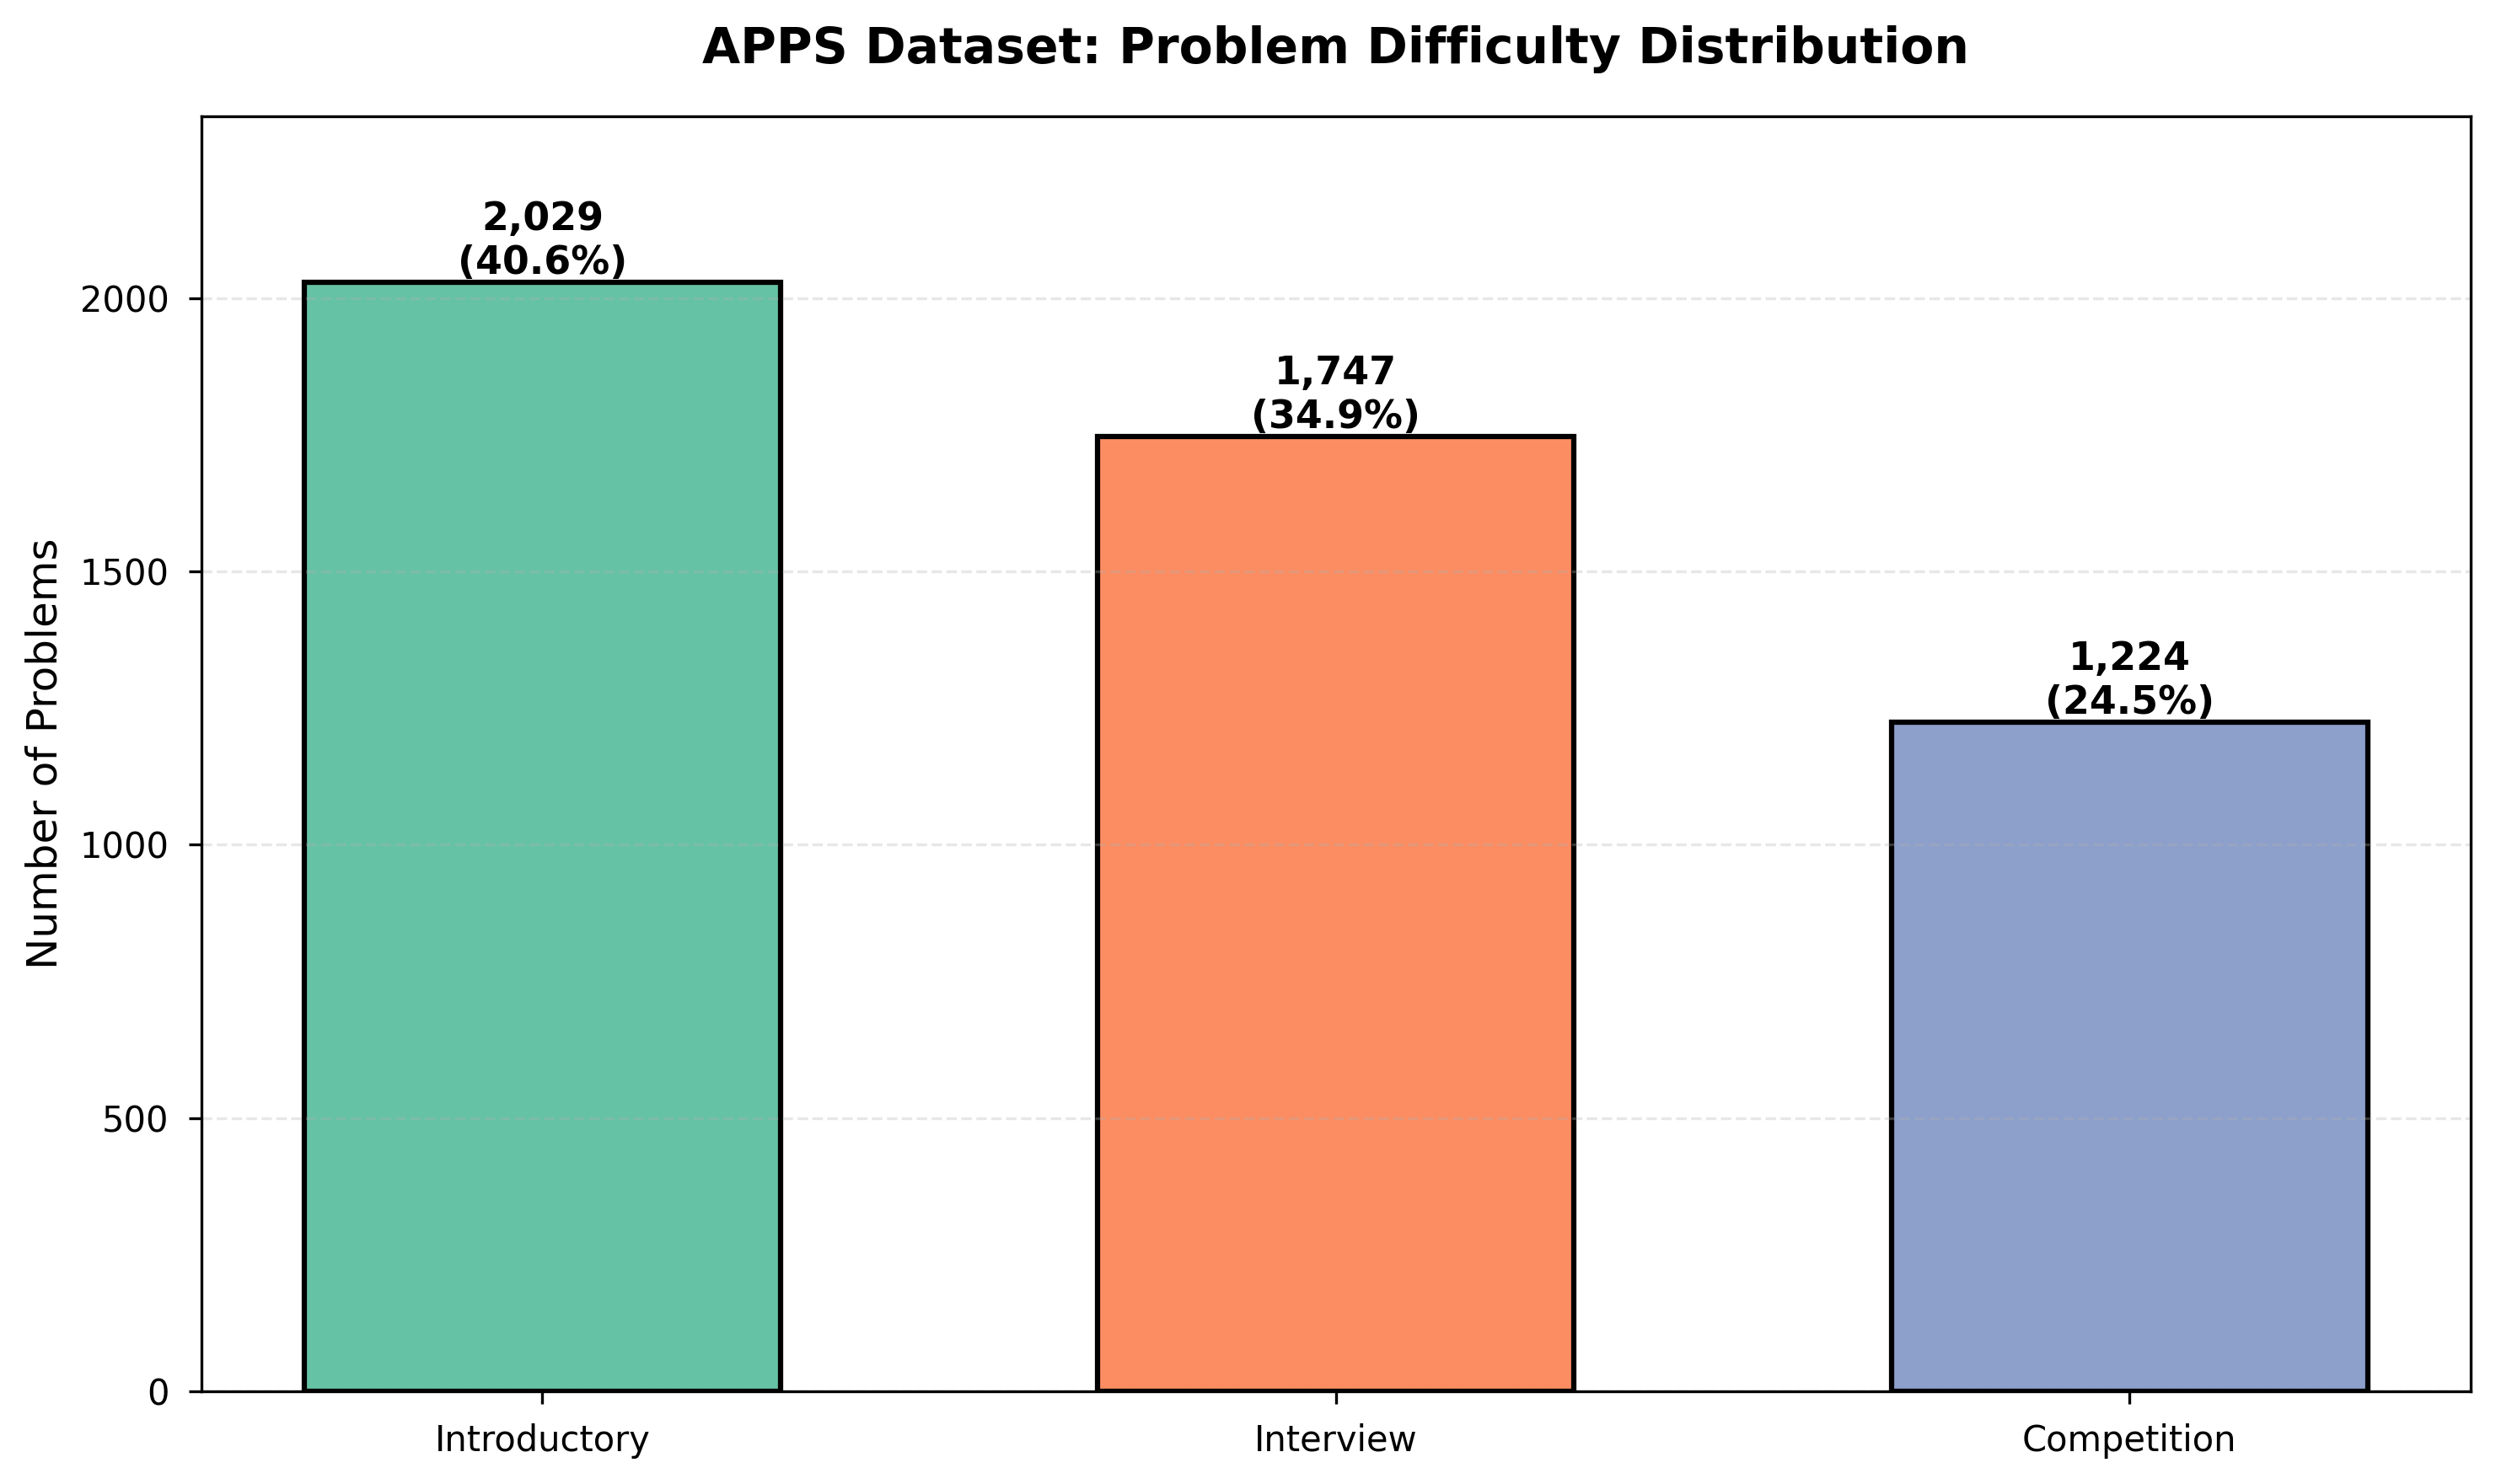
\includegraphics[width=0.8\textwidth]{difficulty_distribution.png}
    \caption{APPS Dataset: Problem Difficulty Distribution}
\end{figure}



\section{Milestone 1 Outcome}

By the end of Milestone 1, we have achieved:
\begin{itemize}
\item Clear problem identification and research objectives
\item Literature review and research gap identification
\item Dataset selection and acquisition
\item Exploratory data analysis
\item Evaluation metrics and benchmarks establishment
\end{itemize}

\section{References}

\begin{thebibliography}{00}
\bibitem{anand2024geometry}

A. Anand et al., \textit{Improving Multimodal LLM’s Ability in Geometry Problem Solving, Reasoning, and Multistep Scoring}, arXiv:2412.00846, 2024. \url{https://arxiv.org/abs/2412.00846}

\bibitem{chen2021codex}
M. Chen et al., \textit{Evaluating Large Language Models Trained on Code}, arXiv:2107.03374, 2021. \url{https://arxiv.org/abs/2107.03374}

\bibitem{roziere2023codellama}
B. Rozière et al., \textit{Code Llama: Open Foundation Models for Code}, arXiv:2308.12950, 2023. \url{https://arxiv.org/abs/2308.12950}

\bibitem{li2023starcoder}
R. Li et al., \textit{StarCoder: May the Source Be With You!}, arXiv:2305.06161, 2023. \url{https://arxiv.org/abs/2305.06161}

\bibitem{sanh2019distilbert}
V. Sanh et al., \textit{DistilBERT, a distilled version of BERT}, arXiv:1910.01108, 2019. \url{https://arxiv.org/abs/1910.01108}

\bibitem{jiao2020tinybert}
X. Jiao et al., \textit{TinyBERT: Distilling BERT for Natural Language Understanding}, Findings of EMNLP 2020. \url{https://aclanthology.org/2020.findings-emnlp.372/}

\bibitem{gunasekar2023phi}
S. Gunasekar et al., \textit{Textbooks Are All You Need}, arXiv:2306.11644, 2023. \url{https://arxiv.org/abs/2306.11644}

\bibitem{feng2020codebert}
Z. Feng et al., \textit{CodeBERT: A Pre-Trained Model for Programming and Natural Languages}, Findings of EMNLP 2020. \url{https://aclanthology.org/2020.findings-emnlp.139/}

\bibitem{xu2022polycoder}
F. Z. Xu et al., \textit{A Systematic Evaluation of Large Language Models of Code}, arXiv:2202.13169, 2022. \url{https://arxiv.org/abs/2202.13169}

\end{thebibliography}

\end{document}